\documentclass[t,9pt,compress=false,usepdftitle=false]{beamer}

\usetheme{default}
%\setbeamercovered{dynamic} % shows items in white grey before active

%no navigational bars:
\setbeamertemplate{navigation symbols}{}

\usepackage[utf8x]{inputenc}
\usepackage[ngerman]{babel}
\usepackage{listings}   % syntax highlighting
\usepackage{courier}
\usepackage{xcolor}
\usepackage{verbatim}

% http://stackoverflow.com/questions/1662037/how-to-write-programming-code-containing-the-character-in-latex
\makeatletter
\let \@sverbatim \@verbatim
\def \@verbatim {\@sverbatim \verbatimplus}
{\catcode`'=13 \gdef \verbatimplus{\catcode`'=13 \chardef '=13 }} 
\makeatother


%\usepackage{amsmath}
%\usepackage{amssymb}

% -----------------------------------------------------------------------------
%
%\newtheorem{definition}{Definition}
\newcommand{\foot}[1]{_{\mbox{\footnotesize #1}}}
\newcommand{\head}[1]{^{\mbox{\footnotesize #1}}}
%
%
\newcommand{\ones}{\mathbb{I}}
\newcommand{\nat}{\mathbb{N}}
\newcommand{\real}{\mathbb{R}}
\newcommand{\ganz}{\mathbb{Z}}
%
%
\newcommand{\RRE}{\mbox{RRE}}
\newcommand{\nnz}[1]{\mbox{nnz}(#1)}
\newlength{\Hoehe}
\renewcommand{\vec}[1]{#1}
\newlength{\GLaenge}
\setlength{\GLaenge}{3.5cm}
%
%
\definecolor{MyGrey}{gray}{0.45}
\def\bstheta{\boldsymbol{\theta}}
\def\bsalpha{\boldsymbol{\alpha}}
\def\bsk{\boldsymbol{k}}
\def\bsx{\boldsymbol{x}}
\def\bsh{\boldsymbol{h}}
%
% Centred minipage environment
%
\newenvironment{cmpage}[1]{
\begin{center}
\begin{minipage}{#1\textwidth}}%
{\end{minipage}\end{center}}
%
%
\newcommand{\POS}{\color{blue}\item [\boldmath{$+$}]}
\newcommand{\NEG}{\color{red}\item [{\boldmath$-$}]}
\newcommand{\NTR}{\color{black}\item [$\circ$]}
\newcommand{\f}[1]{\mathfrak{#1}}
\newcommand{\old}{^{\mbox{\small \color{blue} old}}}
\newcommand{\new}{^{\mbox{\small \color{red} new}}}
\newcommand{\diag}[1]{\mbox{diag}\left(#1\right)}
%
%
\newcommand{\myBlank}{\textvisiblespace}
\newcommand{\noSpace}{\makebox[0pt]{\quad}}
%
% Old style colour commands
%
\newcommand{\CB}{\color{blue}}
\newcommand{\CR}{\color{red}}
\newcommand{\CG}{\color{green}}
\newcommand{\CC}{\color{cyan}}
%
\definecolor{myWhite}{rgb}{1.00,1.00,1.00}  % real white
\definecolor{myGrey}{rgb}{0.78,0.83,0.94}   % 'light grey blue'
\definecolor{myYellow}{rgb}{1.00,1.00,0.00} % yellow
\definecolor{myOrange}{rgb}{1.00,0.65,0.00} % orange
\definecolor{myCyan}{rgb}{0.00,1.00,1.00}   % cyan
%
% Some abbrevs for setting brief code parts
%
\newcommand{\ttA}{\mbox{\texttt{A}}}
\newcommand{\ttB}{\mbox{\texttt{B}}}
\newcommand{\ttC}{\mbox{\texttt{C}}}
\newcommand{\ttD}{\mbox{\texttt{D}}}
\newcommand{\code}[1]{\mbox{\texttt{#1}}}
\newcommand{\ccode}[1]{\cemphd{\texttt{#1}}}
%
% Commands for slides taken from 'Insides'
%
\newcommand{\rst}{\textcolor{emphcolora}{\ast}}
\newcommand{\bst}{\textcolor{emphcolorb}{\ast}}
%
%
%
\definecolor{textcolor} {rgb}{0,0,0}
\definecolor{decocolor} {rgb}{0,0,0}
\definecolor{emphcolora}{rgb}{1,0,0}              % pure red
\definecolor{emphcolorb}{rgb}{0,0,1}              % pure blue
\definecolor{emphcolorc}{cmyk}{0,1,0,0}           % pure magenta
%\definecolor{emphcolord}{cmyk}{0.64,0,0.95,0.20} % sort of green
\definecolor{emphcolord}{rgb}{0,0.4,0.12}         % same as lmu@darkgreen
\definecolor{emphcolore}{cmyk}{1,0,0,0}           % pure cyan
\definecolor{linkcolor} {rgb}{0,0,0}
%
% Commands emphasising text using color
%
\newcommand{\cempha}[1]{{\color{emphcolora}#1}}
\newcommand{\cemphb}[1]{{\color{emphcolorb}#1}}
\newcommand{\cemphc}[1]{{\color{emphcolorc}#1}}
\newcommand{\cemphd}[1]{{\color{emphcolord}#1}}
\newcommand{\cemphe}[1]{{\color{emphcolore}#1}}
\newcommand{\cemphf}[1]{{\color{decocolor}#1}}
% -----------------------------------------------------------------------------
% myColorBox
% -----------------------------------------------------------------------------
\setbeamercolor{myBoxColor}{fg=black,bg=white}
\setbeamercolor{myBoxColorHead}{fg=red,bg=white}
% \newenvironment{myColorBox}[2]{%
% \begin{beamerboxesrounded}[shadow=true,lower=myBoxColor,upper=myBoxColorHead,
% width=#1\textwidth]{#2}}%
% {\end{beamerboxesrounded}}
\newenvironment{myColorBox}[2]{%
\begin{cmpage}{#1}%
\begin{beamerboxesrounded}[shadow=true,lower=myBoxColor,upper=myBoxColorHead]%
{#2}}%
{\end{beamerboxesrounded}\end{cmpage}}
%
% -----------------------------------------------------------------------------
% Math Operators, alternate greek symbols and the like
% -----------------------------------------------------------------------------
\DeclareMathOperator{\grad}{grad}
\DeclareMathOperator{\mydiv}{div}
\DeclareMathOperator{\Grad}{grad}
\DeclareMathOperator{\Div}{div}
%\newcommand{\grad}{\mbox{grad}}
%\newcommand{\mydiv}{\mbox{div}}
\renewcommand{\rho}{\varrho}
%
% -----------------------------------------------------------------------------
% Some color defintions to be compatible with XFIG
% -----------------------------------------------------------------------------
%
\definecolor{XFIGgold}{rgb}{1.00,0.84,0.00}
\definecolor{XFIGltblue}{rgb}{0.53,0.81,1.00}
\definecolor{XFIGred}{rgb}{1.00,0.00,0.00}
% -----------------------------------------------------------------------------

%\includeonly{lecture1}

\hypersetup{pdfpagemode=FullScreen}
\hypersetup{breaklinks=false}
\hypersetup{colorlinks=true}
\hypersetup{urlcolor=blue}

\title[Python Intro]{\parbox[c][][c]{0.7\paperwidth}{\centering ObsPy workshop
2012\\
Python Introduction}}
%\author[blub]{blub}
\date[Zurich 2012-09-06]{2012-09-06}
%\institute{quark}

\begin{document}
\lstset{%
language=Python,          % choose the language of the code
basicstyle=\footnotesize, % the size of the fonts that are used for the code
numbers=none,             % where to put the line-numbers
numberstyle=\footnotesize,% the size of the fonts that are used for the line-numbers
stepnumber=1,             % step between line-numbers. For 1 each line will be numbered
numbersep=5pt,            % how far the line-numbers are from the code
%backgroundcolor=\color{white}, % choose the background color.
showspaces=false,         % show spaces adding particular underscores
showstringspaces=false,   % underline spaces within strings
showtabs=false,           % show tabs within strings adding particular underscores
frame=none,               % e.g. single, adds a frame around the code
tabsize=2,                % sets default tabsize to 2 spaces
captionpos=b,             % sets the caption-position to bottom
breaklines=true,          % sets automatic line breaking
breakatwhitespace=false,  % sets if automatic breaks should only happen at whitespace
escapeinside={\%*}{*)},    % if you want to add a comment within your code
%keywordstyle=\color{red}\bfseries\emph,
}
\maketitle
\begin{frame}[fragile]
\frametitle{Program Thursday}
\begin{tabbing}
\textbf{Morning}: \= Python data types, flow control, file i/o, functions,
modules, classes, errors and exceptions, plotting \kill
\textbf{Morning}: \= Introduction to Python data types, flow control, file i/o,
functions,\\
 modules, classes, errors and exceptions, plotting + exercises \\
\\
\textbf{Afternoon}: \= Introduction to numpy, scipy, basemap, pyproj and quakepy
+ exercises
\\
\\ 
\textbf{Coffee breaks} at 10:30am and 3pm\\
\textbf{Lunch break} from 12:00pm to 1pm\\
\end{tabbing}
\end{frame}

\begin{frame}[fragile]
    \frametitle{Outline}
    \begin{itemize}
        \item This course will \textbf{not} teach you basic programming
        \item Assume you already know:
        \begin{itemize}
            \item variables
            \item loops
            \item conditionals (if / else)
            \item standard data types, int, float, string, lists / arrays
            \item reading/writing data from files
        \end{itemize}
        \item We will:
        	\begin{itemize}
        	  \item show you how to use these in Python 
		      \item present some important concepts when using numpy arrays
		      \item present a few modules in numpy and scipy
		      \item give a few examples on how to plot graphs and maps
        	\end{itemize} 
    \end{itemize}
\end{frame}

\begin{frame}[fragile]
    \frametitle{A few reasons for using Python for Research}
    \begin{enumerate}
        \item Readability
        \item Batteries included
        \item Speed
        \item Language Interoperability
    \end{enumerate}
\end{frame}


\begin{frame}[fragile]
    \frametitle{Readability}
    Guido van Rossum (Python's original author)
        \begin{quote}
This emphasis on readability is no accident. As an object-oriented language, Python aims to encourage the creation of reusable code. Even if we all wrote perfect documentation all of the time, code can hardly be considered reusable if it's not readable. Many of Python’s features, in addition to its use of indentation, conspire to make Python code highly readable.
    \end{quote}
\end{frame}

\begin{frame}[fragile]
    \frametitle{''Batteries included''}
    \begin{itemize}
        \item Extensive standard libraries:
        \begin{itemize}
            \item Data Compression and Archiving
            \item Cryptographic Services
            \item Internet Protocols
            \item Internet Data Handling
            \item Structured Markup Processing Tools
            \item Multimedia Services
            \item Internationalization
            \item Development Tools
            \item Multithreading \& Multiprocessing
            \item Regular expressions
            \item Graphical User Interfaces with Tk
            \item ...
        \end{itemize}
    \end{itemize}
\end{frame}

\begin{frame}[fragile]
    \frametitle{IPython}
    \begin{itemize}
        \item Enhanced interactive Python shell
        \item Main features
        \begin{itemize}
            \item Dynamic introspection and help
            \item Searching through modules and namespaces
            \item Tab completion
            \item Complete system shell access
            \item Session logging \& restoring
            \item Verbose and colored exception traceback printouts
            \item Highly configurable, programmable (Macros, Aliases)
            \item Embeddable
        \end{itemize}
    \end{itemize}
\end{frame}

\begin{frame}[fragile]
    \frametitle{IPython: Getting Help}
    \begin{itemize}
    \item Get help for a function:
    \begin{myColorBox}{0.9}{} \verb#>>> command?#\end{myColorBox}
    \item Have a look at the implementation:
    \begin{myColorBox}{0.9}{} \verb#>>> command??#\end{myColorBox}
    \item Search for variables/functions/modules starting with 'ab':
    \begin{myColorBox}{0.9}{} \verb#>>> ab<Tab>#\end{myColorBox}
    \item Which objects are assigned anyway? 
    \begin{myColorBox}{0.9}{} \verb#>>> whos#\end{myColorBox}
    \item What attributes/methods are there? 
    \begin{myColorBox}{0.9}{}\verb#>>> object.<Tab>#\end{myColorBox}
    \item Get help for a object/class method/attribute:
    \begin{myColorBox}{0.9}{} \verb#>>> object.command?#\end{myColorBox}
    \end{itemize}
\end{frame}

\begin{frame}[fragile]
    \frametitle{Python Data Types: Numbers}
    \begin{myColorBox}{0.9}{}
\begin{verbatim}
>>> a = 17
>>> type(a)
<type 'int'>
\end{verbatim}
    \end{myColorBox}
    \pause
    \begin{myColorBox}{0.9}{}
\begin{verbatim}
>>> a / 10
1
>>> a % 10
7
>>> a / 10.0
1.7
\end{verbatim}
    \end{myColorBox}
    \pause
    \begin{myColorBox}{0.9}{}
\begin{verbatim}
>>> _
1.7
>>> type(_)
<type 'float'>
\end{verbatim}
    \end{myColorBox}
\end{frame}


\begin{frame}[fragile]
    \frametitle{Python Data Types: Numbers}
    \begin{myColorBox}{0.91}{}
\begin{verbatim}
>>> x = y = z = 0
\end{verbatim}
    \end{myColorBox}
    \pause
    \begin{myColorBox}{0.91}{}
\begin{verbatim}
>>> a=3.0+4.0j
>>> float(a)
Traceback (most recent call last):
\dots
TypeError: can't convert complex to float
>>> a.real
3.0
>>> a.imag
4.0
>>> abs(a)  # sqrt(a.real**2 + a.imag**2)
5.0
\end{verbatim}
    \end{myColorBox}
\end{frame}


\begin{frame}[fragile]
    \frametitle{Python Data Types: Numbers}
    \begin{myColorBox}{0.9}{}
\begin{verbatim}
>>> a = 17
>>> a = a + 1
>>> a
18
\end{verbatim}
    \end{myColorBox}
    \pause
    \begin{myColorBox}{0.9}{}
\begin{verbatim}
>>> a+=2
>>> a
20
\end{verbatim}
    \end{myColorBox}
    \pause
    \begin{myColorBox}{0.9}{}
\begin{verbatim}
>>> a++
     a++
        ^
SyntaxError: invalid syntax
\end{verbatim}
    \end{myColorBox}
\end{frame}

\begin{frame}[fragile]
    \frametitle{Python Data Types: Strings}
    \begin{myColorBox}{0.9}{}
\begin{verbatim}
>>> 'spam eggs'
'spam eggs'
>>> "doesn't"
"doesn't"
\end{verbatim}
    \end{myColorBox}
    \pause
    \begin{myColorBox}{0.9}{}
\begin{verbatim}
>>> 'doesn\'t'
"doesn't"
>>> '"Yes," he said.'
'"Yes," he said.'
>>> "\"Yes,\" he said."
'"Yes," he said.'
>>> '"Isn\'t," she said.'
'"Isn\'t," she said.'
\end{verbatim}
    \end{myColorBox}
\end{frame}


\begin{frame}[fragile]
    \frametitle{Python Data Types: Strings}
    \begin{myColorBox}{0.9}{}
\begin{verbatim}
>>> hello = "This is a rather long string\n\
... containing several lines of text.\n\
...     Note that whitespace at the beginning of \
...  the line is significant."
\end{verbatim}
    \end{myColorBox}
    \pause
    \begin{myColorBox}{0.9}{}
\begin{verbatim}
>>> print """
... Usage: thingy [OPTIONS]
...      -h                Display this message
...      -H hostname       Hostname to connect to
... """
\end{verbatim}
    \end{myColorBox}
\end{frame}


\begin{frame}[fragile]
    \frametitle{Python Data Types: Strings}
    \begin{myColorBox}{0.9}{}
\begin{verbatim}
>>> ’sp’ + ’am’
’spam’
>>> ’spam’ * 10
’spamspamspamspamspamspamspamspamspamspam’
\end{verbatim}
    \end{myColorBox}
    \pause
    \begin{myColorBox}{0.9}{}
\begin{verbatim}
>>> a = "workshop at the SED"
>>> a[0]
'w'
>>> a[0:1]
'w' # different than in other languages!
>>> a[0:8]
'workshop'
>>> a[-3:]
'SED'
\end{verbatim}
    \end{myColorBox}
\end{frame}


\begin{frame}[fragile]
    \frametitle{Python Data Types: Strings}
    \begin{myColorBox}{0.9}{}
\begin{verbatim}
>>> a = 'spam'
>>> a[3] = 'n' # strings are immutable
Traceback (most recent call last):
...
TypeError: 'str' object does not support item assignment
\end{verbatim}
    \end{myColorBox}
    \pause
    \begin{myColorBox}{0.9}{}
\begin{verbatim}
>>> b = a[:-1] + 'n'
>>> b
'span'
\end{verbatim}
    \end{myColorBox}
    \pause
    \begin{myColorBox}{0.9}{}
\begin{verbatim}
>>> len(b)
4
\end{verbatim}
    \end{myColorBox}
\end{frame}


\begin{frame}[fragile]
    \frametitle{Python Data Types: Strings}
    Strings are objects with many useful methods:
    \begin{myColorBox}{0.9}{}
\begin{verbatim}
>>> a = "workshop at the SED"
>>> a.find('at')
9
\end{verbatim}
    \end{myColorBox}
    \pause
    \begin{myColorBox}{0.9}{}
\begin{verbatim}
>>> a.split()
['workshop', 'at', 'the', 'SED']
\end{verbatim}
    \end{myColorBox}
    \pause
    \begin{myColorBox}{0.9}{}
\begin{verbatim}
>>> '*'.join(_)
'workshop*at*the*SED'
\end{verbatim}
    \end{myColorBox}
    There are more useful \verb#string# methods like \verb#startswith#, \verb#endswith#, \verb#lower#, \verb#upper#,
    \verb#ljust#, \verb#rjust#, \verb#center#, \verb#...#. See Python Library Reference.
\end{frame}

\begin{frame}[fragile]
    \frametitle{Python Data Types: Lists}
    \begin{myColorBox}{0.9}{}
\begin{verbatim}
>>> a = ['spam', 'eggs', 100, 1234]
>>> a
['spam', 'eggs', 100, 1234]
\end{verbatim}
    \end{myColorBox}
    \pause
    \begin{myColorBox}{0.9}{}
\begin{verbatim}
>>> a[0]
'spam'
>>> a[3]
1234
>>> a[-2]
100
>>> a[:2] + ['bacon', 2*2]
['spam', 'eggs', 'bacon', 4]
>>> 2*a[:3] + ['Boo!']
['spam', 'eggs', 100, 'spam', 'eggs', 100, 'Boo!']
\end{verbatim}
    \end{myColorBox}
\end{frame}

\begin{frame}[fragile]
    \frametitle{Python Data Types: Lists}
    \begin{myColorBox}{0.9}{}
\begin{verbatim}
>>> a
['spam', 'eggs', 100, 1234]
>>> a[2] = a[2] + 23 # lists are mutable
>>> a
['spam', 'eggs', 123, 1234]
\end{verbatim}
    \end{myColorBox}
    \pause
    \begin{myColorBox}{0.9}{}
\begin{verbatim}
>>> a[0:2] = [1, 12] # Replace some items
>>> a
[1, 12, 123, 1234]
>>> sum(a) # some over all items
1370
>>> a[0:2] = [] # Remove some
>>> a
[123, 1234]
>>> a[1:1] = ['bletch', 'xyzzy'] # Insert some
>>> a
[123, 'bletch', 'xyzzy', 1234]
\end{verbatim}
    \end{myColorBox}
\end{frame}


\begin{frame}[fragile]
    \frametitle{Python Data Types: Lists}
    \begin{myColorBox}{0.9}{}
\begin{verbatim}
>>> a[::-1]
[1234, 'xyzzy', 'bletch', 123]
\end{verbatim}
    \end{myColorBox}
    \pause
    \begin{myColorBox}{0.9}{}
\begin{verbatim}
>>> len(a)
4
\end{verbatim}
    \end{myColorBox}
    \pause
    \begin{myColorBox}{0.9}{}
\begin{verbatim}
>>> a[:] = [] # Clear the list
>>> a
[]
\end{verbatim}
    \end{myColorBox}
    \pause
    There are more useful \verb#list# methods like \verb#append#, \verb#insert#, \verb#remove#, \verb#sort#,
    \verb#pop#, \verb#index#, \verb#reverse#, \verb#...#. See Python Library Reference.
\end{frame}


\begin{frame}[fragile]
    \frametitle{Python Data Types: Tuples, Boolean \& None}
    Tuples
    \begin{itemize}
        \item Immutable lists created by \textbf{round} parantheses
        \item Parantheses can be ommited in many cases.
    \end{itemize}
    \begin{myColorBox}{0.9}{}
\begin{verbatim}
>>> t = (12345, 54321, 'hello!')
>>> t[0]
12345
\end{verbatim}
    \end{myColorBox}
\pause
Boolean
        \begin{myColorBox}{0.9}{}
\begin{verbatim}
>>> type(True)
<type 'bool'>
\end{verbatim}
    \end{myColorBox}
\pause
None
        \begin{myColorBox}{0.9}{}
\begin{verbatim}
>>> a = None
>>> type(a)
<type 'NoneType'>
\end{verbatim}
    \end{myColorBox}
\pause

\end{frame}

\begin{frame}[fragile]
    \frametitle{Python Data Types: Dictionaries}
    \begin{myColorBox}{0.9}{}
\begin{verbatim}
>>> tel = {'jack': 4098, 'sape': 4139}
>>> tel['guido'] = 4127
>>> tel
{'sape': 4139, 'guido': 4127, 'jack': 4098}
>>> tel['jack']
4098
>>> del tel['sape']
>>> tel['irv'] = 4127
>>> tel
{'guido': 4127, 'irv': 4127, 'jack': 4098}
>>> tel.keys()
['guido', 'irv', 'jack']
>>> 'guido' in tel
True
\end{verbatim}
    \end{myColorBox}
\end{frame}

\begin{frame}[fragile]
    \frametitle{Flow Control: if-statement}
    \begin{myColorBox}{0.9}{}
\begin{verbatim}
>>> x = int(raw_input("Please enter an integer: "))
Please enter an integer: 42
>>> if x < 0:
...      print 'Negative'
... elif x == 0:
...      print 'Zero'
... elif x == 1:
...      print 'Single'
... else:
...      print 'More'
...
More
\end{verbatim}
    \end{myColorBox}
\end{frame}


\begin{frame}[fragile]
    \frametitle{Flow Control: for-statement}
    \begin{myColorBox}{0.9}{}
\begin{verbatim}
>>> a = ['cat', 'window', 'defenestrate']
>>> for x in a:
...     print x, len(x)
...
cat 3
window 6
defenestrate 12
\end{verbatim}
    \end{myColorBox}
    \pause
    \begin{myColorBox}{0.9}{}
\begin{verbatim}
>>> for i in range(0, 6, 2):
...     print i
...
0
2
4
\end{verbatim}
    \end{myColorBox}
\end{frame}


\begin{frame}[fragile]
    \frametitle{Flow Control: while-statement}
    \begin{myColorBox}{0.9}{}
\begin{verbatim}
>>> import time
>>> i = 1
>>> while True:
...     i = i * 1000 # same as: i *= 1000
...     print repr(i)
...     time.sleep(1) # wait one second
...
1000
1000000
1000000000
1000000000000L # <- type conversion occured!
1000000000000000L
# ... continues until memory is exhausted!
\end{verbatim}
    \end{myColorBox}
\end{frame}


\begin{frame}[fragile]
    \frametitle{Flow Control: continue \& break}
The \verb#break# statement breaks out of the smallest enclosing for or while loop.
    \begin{myColorBox}{0.9}{}
\begin{verbatim}
>>> for i in range(0, 100000):
...     if i>50:
...         print i
...         break
...
51
\end{verbatim}
    \end{myColorBox}
\pause
The \verb#continue# statement continues with the next iteration of the loop.
    \begin{myColorBox}{0.9}{}
\begin{verbatim}
>>> for i in range(0, 100000):
...     if i!=50:
...         continue
...     print i
...
50
\end{verbatim}
    \end{myColorBox}
\end{frame}


\begin{frame}[fragile]
    \frametitle{File Handling}
    Use \verb#open(filename, mode)# to open a file. Returns a File Object.
    \begin{myColorBox}{0.9}{}
\begin{verbatim}
fh = open('/path/to/file', 'r')
\end{verbatim}
    \end{myColorBox}
   \begin{itemize}
   \item Some possible modes:
   \begin{itemize}
        \item r: Open text file for read.
        \item w: Open text file for write.
        \item a: Open text file for append.
        \item rb: Open binary file for read.
        \item wb: Open binary file for write.
    \end{itemize}
    \end{itemize}
    Use \verb#close()# to close a given File Object.
    \begin{myColorBox}{0.9}{}
\begin{verbatim}
fh.close()
\end{verbatim}
    \end{myColorBox}
\end{frame}

\begin{frame}[fragile]
    \frametitle{Reading Files}
Read a quantity of data from a file:
    \begin{myColorBox}{1.0}{}
\begin{verbatim}
s = fh.read( size ) # size: number of bytes to read
\end{verbatim}
    \end{myColorBox}
\pause
Read entire file
    \begin{myColorBox}{0.9}{}
\begin{verbatim}
s = fh.read()
\end{verbatim}
    \end{myColorBox}
\pause
Read one line from file:
    \begin{myColorBox}{0.9}{}
\begin{verbatim}
s = fh.readline()
\end{verbatim}
    \end{myColorBox}
\pause
Get all lines of data from the file into a list:
    \begin{myColorBox}{0.9}{}
\begin{verbatim}
list = fh.readlines()
\end{verbatim}
    \end{myColorBox}
\pause
Iterate over each line in the file:
    \begin{myColorBox}{0.9}{}
\begin{verbatim}
for line in fh:
    print line,
\end{verbatim}
    \end{myColorBox}
\end{frame}

\begin{frame}[fragile]
    \frametitle{Writing Files}
Write a string to the file:
    \begin{myColorBox}{0.9}{}
\begin{verbatim}
fh.write( string )
\end{verbatim}
    \end{myColorBox}
\pause
Write several strings to the file:
    \begin{myColorBox}{0.9}{}
\begin{verbatim}
fh.writelines( sequence )
\end{verbatim}
    \end{myColorBox}
\end{frame}

\begin{frame}[fragile]
\frametitle{The sys module}
\verb#sys.argv# returns a list of strings with the pathname of the script
as the first entry and the command line arguments as the following entries.
    \begin{myColorBox}{0.9}{}
    \begin{verbatim}
#!/usr/bin/env python
import sys
print sys.argv
    \end{verbatim}
    \end{myColorBox}
    \begin{myColorBox}{0.9}{}
    \begin{verbatim}
In [4]: run tests.py command1 command2
['tests.py', 'command1', 'command2']
    \end{verbatim}
    \end{myColorBox}
    \pause
Get information on your platform:
    \begin{myColorBox}{0.9}{}
    \begin{verbatim}
>>> sys.platform
'linux2'
    \end{verbatim}
    \end{myColorBox}
\end{frame}

\begin{frame}[fragile]
\frametitle{The sys module}
\verb#sys.path# returns the module search path as a list of strings. 
    \begin{myColorBox}{0.9}{}
    \begin{verbatim}
>>> sys.path
['','/usr/lib/python2.7', 
'/usr/local/src/obspy_git/trunk/obspy.core',
 ...]
    \end{verbatim}
    \end{myColorBox}
    \pause
If you have written a python module \verb#mymodule.py# that is located in
\verb#/my/path/# and you want to load it into another script you could do the
following:
    \begin{myColorBox}{0.9}{}
    \begin{verbatim}
>>> sys.path.append('/my/path/')
>>> import mymodule
    \end{verbatim}
    \end{myColorBox}
\end{frame}

\begin{frame}
\begin{center}
\Huge{Exercises}
\end{center}
\end{frame}

\begin{frame}
\begin{center}
\Huge{Functions, modules, classes, exceptions and plotting}
\end{center}
\end{frame}

\begin{frame}
    \begin{center}
    \Huge{Functions}
    \end{center}
\end{frame}

\begin{frame}[fragile]
    \frametitle{Functions}
Defining a function which returns a Fibonacci series up to n.
    \begin{myColorBox}{0.9}{}
\begin{verbatim}
>>> def fib(n):
...     """Return the Fibonacci series up to n."""
...     result = []
...     a, b = 0, 1
...     while a < n:
...         result.append(a)
...         a, b = b, a+b
...     return result
\end{verbatim}
    \end{myColorBox}
\pause
Now call the function we just defined:
    \begin{myColorBox}{0.9}{}
\begin{verbatim}
>>> fib(100)
[0, 1, 1, 2, 3, 5, 8, 13, 21, 34, 55, 89]
\end{verbatim}
    \end{myColorBox}
\end{frame}

\begin{frame}[fragile]
    \frametitle{Functions}
    \begin{myColorBox}{0.9}{}
\begin{verbatim}
def birthday2(name, age = 1):
    msg = "Happy birthday, %s! You're %d today."
    print  msg % (name, age)
\end{verbatim}
    \end{myColorBox}
\pause
    \begin{myColorBox}{0.9}{}
\begin{verbatim}
>>> birthday2("Katherine")
Happy birthday, Katherine! You're 1 today.
\end{verbatim}
    \end{myColorBox}
\pause
    \begin{myColorBox}{0.9}{}
\begin{verbatim}
>>> birthday2(age = 12, name = "Katherine")
Happy birthday, Katherine! You're 12 today.
\end{verbatim}
    \end{myColorBox}
\pause
    \begin{myColorBox}{0.9}{}
\begin{verbatim}
>>> birthday2("Katherine", 14)
Happy birthday, Katherine! You're 14 today.
\end{verbatim}
    \end{myColorBox}
\end{frame}

\begin{frame}
    \begin{center}
    \Huge{Modules}
    \end{center}
\end{frame}

\begin{frame}[fragile]
    \frametitle{Modules}
Importing functionality of a module the normal and safe way:
    \begin{myColorBox}{0.9}{}
\begin{verbatim}
>>> import math
>>> math.pi
3.141592653589793
>>> math.cos(math.pi)
-1.0
\end{verbatim}
    \end{myColorBox}
\pause
Importing directly into the local namespace:
    \begin{myColorBox}{0.9}{}
\begin{verbatim}
>>> from math import *
>>> pi
3.141592653589793
>>> cos(pi)
-1.0
\end{verbatim}
    \end{myColorBox}
\end{frame}

\begin{frame}[fragile]
\frametitle{Modules}
Caution with \verb#from module import *#
    \begin{myColorBox}{0.9}{}
\begin{verbatim}
>>> from os import *
>>> f = open('Makefile','r')
Traceback (most recent call last):
  File "<stdin>", line 1, in <module>
TypeError: an integer is required

# open() has been mapped to os.open() !!!
\end{verbatim}
\end{myColorBox}
The builtin open() could still be accessed though:
\begin{myColorBox}{0.9}{}
\begin{verbatim}
>>> f = __builtins__.open('Makefile','r')
\end{verbatim}
\end{myColorBox}
\end{frame}

\begin{frame}[fragile]
\frametitle{Modules}
Less typing while avoiding collisions by binding to local names
\begin{myColorBox}{0.9}{}
\begin{verbatim}
>>> import math
>>> cos = math.cos
>>> pi = math.pi
>>> cos(pi)
-1.0
\end{verbatim}
\end{myColorBox}

Import module under a different/shorter name:
\begin{myColorBox}{0.9}{}
\begin{verbatim}
>>> import math as m
>>> m.cos(m.pi)
-1.0
\end{verbatim}
\end{myColorBox}

Import only what is needed:
\begin{myColorBox}{0.9}{}
\begin{verbatim}
>>> from math import pi, cos
>>> cos(pi)
-1.0
\end{verbatim}
\end{myColorBox}
\end{frame}

\begin{frame}[fragile]
\frametitle{Modules}
Writing your own module called \verb#seismo.py#:
\begin{verbatim}
"""Some seismological utility functions."""

import math

def lame_parameters(alpha, beta, density):
    """ Convert seismic velocities to Lame's parameters.
        Returns Lame's parameters as (lambda, mu)."""
    return ((alpha ** 2 - 2.0 * beta ** 2) * density,
            beta ** 2 * density)

def velocities(lambd, mu, density):
    """ Convert lame parameters to seismic velocities.
        Returns tuple with velocities (alpha, beta). """
    return (math.sqrt((lambd + 2.0 * mu) / density),
            math.sqrt(mu / density))
\end{verbatim}
\end{frame}

\begin{frame}[fragile]
\frametitle{Modules}
Using your module as any other module:
\begin{myColorBox}{0.9}{}
\begin{verbatim}
>>> import seismo
>>> seismo.lame_parameters(4000., 2100., 2600.)
(18668000000.0, 11466000000.0)
>>> _
(18668000000.0, 11466000000.0)
>>> (_+(2600,))
(18668000000.0, 11466000000.0, 2600)
>>> seismo.velocities(*(_+(2600,)))
(4000.0, 2100.0)
\end{verbatim}
\end{myColorBox}
\end{frame}

\begin{frame}[fragile]
\frametitle{Modules}
Help!
\begin{myColorBox}{1.0}{}
\begin{verbatim}
>>> import seismo
>>> help(seismo)
\end{verbatim}
\end{myColorBox}
\begin{myColorBox}{1.0}{}
\begin{verbatim}
Help on module seismo:

NAME
    seismo - Some seismological utility functions.

FILE
    /obspy_git/branches/docs/sed_2012/seismo.py

FUNCTIONS
    lame_parameters(alpha, beta, density)
        Convert seismic velocities to Lame's parameters.
        Returns Lame's parameters as (lambda, mu).
    
    velocities(lambd, mu, density)
        Convert lame parameters to seismic velocities.
        Returns tuple with velocities (alpha, beta).

\end{verbatim}
\end{myColorBox}
\end{frame}

\begin{frame}[fragile]
\frametitle{Modules}
You can look at the contents of any module
\begin{myColorBox}{0.9}{}
\begin{verbatim}
>>> import seismo
>>> dir(seismo)
['__builtins__', '__doc__', '__file__', 
'__name__', '__package__', 'lame_parameters', 
'math', 'velocities']

\end{verbatim}
\end{myColorBox}
\verb#dir# without argument looks at local namespace
\begin{myColorBox}{0.9}{}
\begin{verbatim}
... 
>>> dir()
['__builtins__', '__doc__',
 '__name__', '__package__', 'seismo']
\end{verbatim}
\end{myColorBox}
\end{frame}

\begin{frame}
    \begin{center}
    \Huge{Errors and Exceptions}
    \end{center}
\end{frame}

\begin{frame}[fragile]
    \frametitle{Errors and Exceptions}
    \begin{myColorBox}{1.0}{}
\begin{verbatim}
>>> 10 * (1/0)
Traceback (most recent call last):
  File "<stdin>", line 1, in ?
ZeroDivisionError: integer division or modulo by zero
\end{verbatim}
    \end{myColorBox}
    \pause    
    \begin{myColorBox}{1.0}{}
\begin{verbatim}
>>> 4 + muh*3
Traceback (most recent call last):
  File "<stdin>", line 1, in ?
NameError: name 'muh' is not defined
\end{verbatim}
    \end{myColorBox}
    \pause    
    \begin{myColorBox}{1.0}{}
\begin{verbatim}
>>> '2' + 2
Traceback (most recent call last):
  File "<stdin>", line 1, in ?
TypeError: cannot concatenate 'str' and 'int' objects
\end{verbatim}
    \end{myColorBox}
\end{frame}


\begin{frame}[fragile]
    \frametitle{Errors and Exceptions}
Handling Exceptions:
    \begin{myColorBox}{1.0}{}
\begin{verbatim}
def divide(x, y):
    try:
        result = x / y
    except ZeroDivisionError:
        print "division by zero!"
    except TypeError:
        print "unsupported type!"
    else:
        print "result is", result
\end{verbatim}
    \end{myColorBox}
    \begin{myColorBox}{1.0}{}
\begin{verbatim}
>>> divide(2, 1)
result is 2
>>> divide(2, 0)
division by zero!
>>> divide(2, 'bbb')
unsupported type!
\end{verbatim}
    \end{myColorBox}
\end{frame}

\begin{frame}[fragile]
\frametitle{Errors and Exceptions}
More generic Exception handling:
\begin{myColorBox}{1.0}{}
\begin{verbatim}
def divide(x, y):
    try:
        result = x / y
    except Exception, e:
        print "Generic exception! ", e
    else:
        print "result is", result
\end{verbatim}
\end{myColorBox}
    \begin{myColorBox}{1.0}{}
    \begin{verbatim}
>>> divide(3.,'blub')
Generic exception!  unsupported operand type(s) 
for /: 'float' and 'str'

>>> divide(3.,0)
Generic exception!  float division by zero
 
\end{verbatim}
\end{myColorBox}
\end{frame}

\begin{frame}
    \begin{center}
    \Huge{Classes}
    \end{center}
\end{frame}


\begin{frame}[fragile]
    \frametitle{Classes}
    Classes consist of..
    \begin{itemize}
    \item Attributes: Variables that store information about the class' current
    state
    \item Methods: Functions that allow interactions with the class
    \end{itemize}
    Some advantages of using classes..
    \begin{itemize}
    \item Classes know how to behave by themselves
    \item Users do not need to know the details of the class implementation
    \item Programs using the classes get shorter and far more readable
    \end{itemize}
\end{frame}

\begin{frame}[fragile]
\frametitle{Classes}
Syntax:
\begin{itemize}
  \item The \verb#class# keyword introduces a class
  \item To create an instance of the class, use function notation
  \item The \verb#__init__()# method is invoked when an instance of the class is
  created
  \item Class methods receive a reference to the instance as first argument. By
  convention it is called \verb#self#
  \item An \textit{instance object} is an entity encapsulating state (data
  attributes) and behaviour (methods)
  \item A \textit{class} is the blueprint from which individual objects
  (\textit{instances}) are created.
\end{itemize}
\end{frame}

\begin{frame}[fragile]
    \frametitle{Classes}
Example:
    \begin{myColorBox}{0.9}{}
\small
\begin{verbatim}
class Rectangle:
    def __init__(self,x,y):
        self.x = x
        self.y = y

    def area(self):
        return self.x * self.y
\end{verbatim}
    \end{myColorBox}
    \begin{myColorBox}{0.9}{}
\small
\begin{verbatim}
>>> r = Rectangle(10,20)
>>> r.area()
200
\end{verbatim}
    \end{myColorBox}
\end{frame}

\begin{frame}[fragile]
\frametitle{Classes}
Inheritance
\begin{itemize}
  \item Motivation: add functionality but reuse existing code
  \item A derived class has all the attributes and methods from the base class
  but can add new attributes and methods
  \item If any new attributes or methods have the same name as an attribute or
  method in the base class, it is used instead of the base class version.
  \item The syntax is simply \verb#class DerivedClass(BaseClass): ...#
\end{itemize}
\end{frame}

\begin{frame}[fragile]
\frametitle{Classes}
Example:
\begin{myColorBox}{0.9}{}
\begin{verbatim}
class Square(Rectangle):
    def __init__(self,x):
        self.x = x
        self.y = x
\end{verbatim}
\end{myColorBox}
\begin{myColorBox}{0.9}{}
\begin{verbatim}
>>> s = Square(5)
>>> s.area()
25
\end{verbatim}
\end{myColorBox}
\end{frame}

\begin{frame}
    \begin{center}
    \Huge{Plotting}
    \end{center}
\end{frame}

\begin{frame}[fragile]
    \frametitle{Plotting}
Matplotlib is \emph{the} plotting library for Python.
\begin{itemize}
\item syntax is close to Matlab's plotting commands
\item advanced users can control all details of the plots
\end{itemize}
We need to import \verb#matplotlib# for the following examples:
\begin{myColorBox}{0.9}{}
\begin{verbatim}
>>> import matplotlib.pyplot as plt
>>> x = [0, 2, 2.5]
>>> plt.plot(x)
[<matplotlib.lines.Line2D object at 0x3372e10>]
>>> plt.show()
\end{verbatim}
    \end{myColorBox}
\pause
\begin{center}
      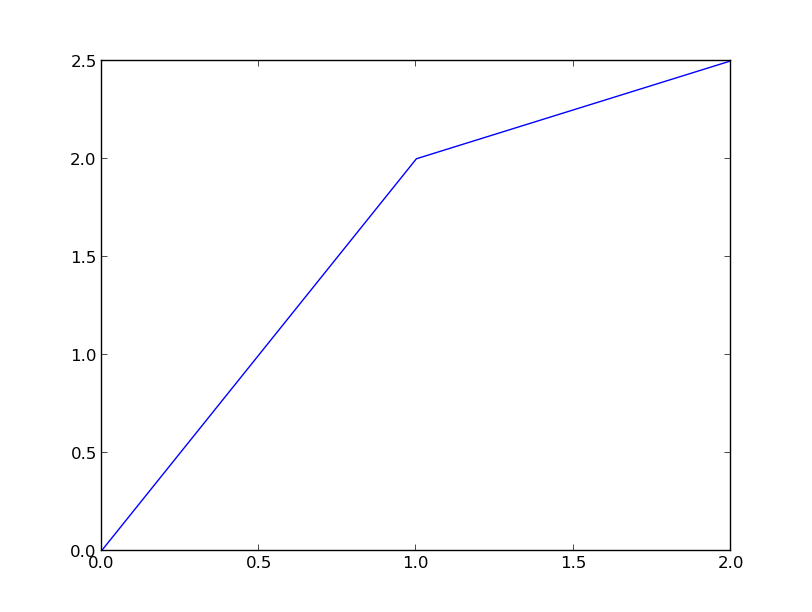
\includegraphics[width=0.4\textwidth]{pix/matplotlib_example_1}
    \end{center}
\end{frame}

\begin{frame}[fragile]
	\frametitle{Plotting}
    \begin{myColorBox}{0.9}{}
\begin{verbatim}
>>> x = [0, 2, 2.5]
>>> y = [1, 2.5, 3.5]
>>> plt.plot(x, y, 'ro')
>>> plt.xlim(-1, 3)
>>> plt.ylim(0, 4)
>>> plt.show()
\end{verbatim}
    \end{myColorBox}
\pause
\begin{center}
      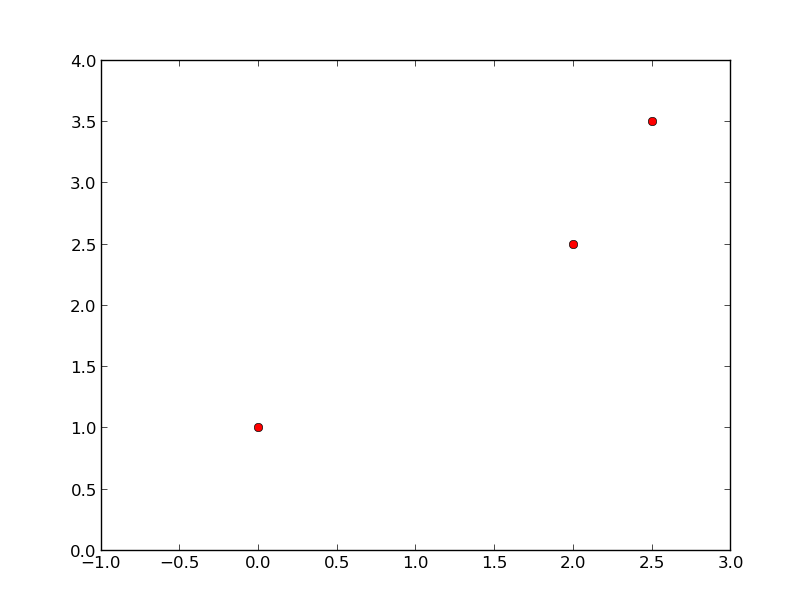
\includegraphics[width=0.6\textwidth]{pix/matplotlib_example_2}
\end{center}
\end{frame}

\begin{frame}[fragile]
    \frametitle{Plotting}
    \begin{myColorBox}{0.9}{}
\begin{verbatim}
>>> import math
>>> t = [0.1 * i for i in range(0,20)]
>>> s = [math.sin(2*math.pi*x) for x in t]
>>> plt.plot(t, s, linewidth=1.0)
>>> plt.xlabel('time (s)')
>>> plt.ylabel('voltage (mV)')
>>> plt.title('This is a very simple plot')
>>> plt.grid(True)
>>> plt.show()
\end{verbatim}
    \end{myColorBox}
\pause
\begin{center}
      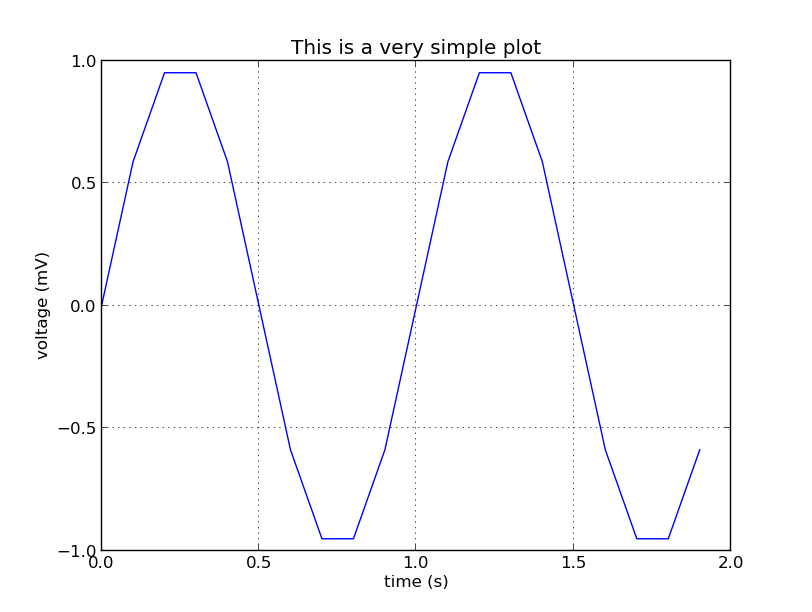
\includegraphics[width=0.5\textwidth]{pix/matplotlib_example_3}
\end{center}
\end{frame}

\begin{frame}
\frametitle{Plotting}
See the Matplotlib homepage for basic plotting commands and especially the
Matplotlib Gallery for many plotting examples with source code!\\
\href{http://matplotlib.sourceforge.net/index.html}{http://matplotlib.sourceforge.net/index.html}
\href{http://matplotlib.sourceforge.net/gallery.html}{http://matplotlib.sourceforge.net/gallery.html}
\end{frame}

\begin{frame}
\begin{center}
\Huge{Exercises}
\end{center}
\end{frame}


\begin{frame}
\begin{center}
\Huge{Numpy and Scipy}
\end{center}
\end{frame}

\begin{frame}
\begin{center}
\Huge{Numpy}
\end{center}
\end{frame}

\begin{frame}[fragile]
    \frametitle{NumPy}
We need to import \verb#numpy# for the following examples:
    \begin{myColorBox}{0.9}{}
\begin{verbatim}
import numpy as np 
\end{verbatim}
    \end{myColorBox}
Numpy arrays:
    \begin{myColorBox}{0.9}{}
\begin{verbatim}
>>> a = np.array( [2, 3, 4] )
>>> a
array([2, 3, 4])
>>> type(a) 
<type 'numpy.ndarray'>
\end{verbatim}
    \end{myColorBox}
    \pause
    \begin{myColorBox}{0.9}{}
\begin{verbatim}
>>> b = np.array( [ (1.5, 2, 3), (4, 5, 6) ] )
>>> b
array([[ 1.5,  2. ,  3. ],
       [ 4. ,  5. ,  6. ]])
\end{verbatim}
    \end{myColorBox}
\end{frame}

\begin{frame}[fragile]
    \frametitle{NumPy}
    \begin{myColorBox}{0.9}{}
\begin{verbatim}
>>> b.ndim     # number of dimensions
2
>>> b.shape    # the dimensions
(2, 3)
>>> b.dtype    # the type (8 byte floats)
dtype('float64')
>>> b.itemsize # the size of the type
8
\end{verbatim}
    \end{myColorBox}
    \pause    
    \begin{myColorBox}{0.9}{}
\begin{verbatim}
>>> c = np.array( [ [1, 2], [3, 4] ], dtype=complex )
>>> c
array([[ 1.+0.j,  2.+0.j],
       [ 3.+0.j,  4.+0.j]])
>>> d = np.array( [ [1+3j, 2], [3+2.5j, 4] ],
				 dtype=complex )
array([[ 1.+3.j ,  2.+0.j ],
       [ 3.+2.5j,  4.+0.j ]])
\end{verbatim}
    \end{myColorBox}
\end{frame}

\begin{frame}[fragile]
\frametitle{NumPy}
You can define your own dtypes. Suppose you have the following array of tuples:
\begin{myColorBox}{1.0}{}
\begin{verbatim}
>>> x = np.array([[('Christian', 43887651), 
('John', 90117628)],
[('Martha', 43887651), 
('Stephen', 90117628)]])
>>> x
array([[['Christian', '43887651'],
        ['John', '90117628']],
       [['Martha', '43887651'],
        ['Stephen', '90117628']]], 
      dtype='|S9')
>>> dt = np.dtype({'names':('name','phone'),
'formats':('|S8', 'i8')})
>>> x = np.array([[('Christian', 43887651), 
('John', 90117628)],
[('Martha', 43887651), 
('Stephen', 90117628)]], dtype=dt)
>>> x
array([[('Christia', 43887651), ('John', 90117628)],
       [('Martha', 43887651), ('Stephen', 90117628)]], 
      dtype=[('name', '|S8'), ('phone', '<i8')])
\end{verbatim}
\end{myColorBox}
\end{frame}

\begin{frame}[fragile]
\frametitle{}
\begin{myColorBox}{1.0}{}
\begin{verbatim}
>>> x['name']
array([['Christia', 'John'],
       ['Martha', 'Stephen']], 
      dtype='|S8')
>>> x[0,0]
('Christia', 43887651)
>>> x['phone'][0,0]
43887651
>>> x[1] = ('Julia',11324455)
>>> x
array([[('Christia', 43887651), ('John', 90117628)],
       [('Julia', 11324455), ('Julia', 11324455)]], 
      dtype=[('name', '|S8'), ('phone', '<i8')])
\end{verbatim}
\end{myColorBox}
\end{frame}

\begin{frame}[fragile]
    \frametitle{NumPy}
A more useful example! Suppose you have a file with entries that look like
this:
\begin{verbatim}
CLC -1.175975e+02 3.581574e+01 soil
SLA -1.172833e+02 3.589095e+01 rock
GRA -1.173662e+02 3.699608e+01 soil
TIN -1.182301e+02 3.705422e+01 soil
\end{verbatim}
    \pause    
    \begin{myColorBox}{1.0}{}
\begin{verbatim}
>>> stdat = np.loadtxt('station_data.txt',
dtype={'names':('stname', 'lon', 'lat', 'substrate'),
'formats': ('|S4', 'f8', 'f8', '|S4')})
>>> stdat
array([('CLC', -117.5975, 35.81574, 'soil'),
       ('SLA', -117.2833, 35.89095, 'rock'),
       ('GRA', -117.3662, 36.99608, 'soil'),
       ('TIN', -118.2301, 37.05422, 'soil')], 
      dtype=[('stname', '|S4'), ('lon', '<f8'),
       ('lat', '<f8'), ('substrate', '|S4')])
>>> stdat['stname']
array(['CLC', 'SLA', 'GRA', 'TIN'], 
      dtype='|S4')
>>> stdat['lon']
>>> array([-117.5975, -117.2833, -117.3662, -118.2301])
\end{verbatim}
    \end{myColorBox}
\end{frame}


\begin{frame}[fragile]
    \frametitle{NumPy}
Create arrays:
    \begin{myColorBox}{1.0}{}
\begin{verbatim}
>>> np.zeros( (3, 4) )  # parameter specify the shape
array([[0.,  0.,  0.,  0.],
       [0.,  0.,  0.,  0.],
       [0.,  0.,  0.,  0.]])
>>> np.ones( (2, 3, 4), dtype=int16 ) # dtype specified
array([[[ 1, 1, 1, 1],
        [ 1, 1, 1, 1],
        [ 1, 1, 1, 1]],
       [[ 1, 1, 1, 1],
        [ 1, 1, 1, 1],
        [ 1, 1, 1, 1]]], dtype=int16)
\end{verbatim}
    \end{myColorBox}
Supported data types: bool, uint8, uint16, uint32, uint64, int8, int16, int32, int64, float32, float64, float96, complex64, complex128, complex192 
\end{frame}

\begin{frame}[fragile]
    \frametitle{NumPy}
    \begin{myColorBox}{1.0}{}
\begin{verbatim}
>>> np.empty( (2,3) )
array([[  3.73603959e-262,   ...,   ...],
       [  5.30498948e-313,   ...,   ...]])
\end{verbatim}
    \end{myColorBox}
    \pause
    \begin{myColorBox}{1.0}{}
\begin{verbatim}
>>> np.arange( 10, 30, 5 )
array([10, 15, 20, 25])
>>> np.arange( 0, 2, 0.3 ) # it accepts float arguments
array([ 0. ,  0.3,  0.6,  0.9,  1.2,  1.5,  1.8])
\end{verbatim}
    \end{myColorBox}
    \pause
    \begin{myColorBox}{1.0}{}
\begin{verbatim}
>>> np.linspace( 0, 2, 9 ) # 9 numbers from 0 to 2
array([ 0.  ,  0.25,  0.5 ,  0.75, ...,  2.  ])
>>> x = np.linspace( 0, 2*pi, 100 )
>>> f = np.sin(x)
\end{verbatim}
    \end{myColorBox}
\end{frame}

\begin{frame}[fragile]
\frametitle{Numpy}
Creating grids
\begin{myColorBox}{0.9}{}
\begin{verbatim}
>>> x = np.arange(0.0,1.1,0.1)
>>> y = x
>>> xx, yy = np.meshgrid(x,y)
>>> xx
array([[ 0. ,  0.1,  0.2, ...,  0.8,  0.9,  1. ],
       [ 0. ,  0.1,  0.2, ...,  0.8,  0.9,  1. ],
       [ 0. ,  0.1,  0.2, ...,  0.8,  0.9,  1. ],
       ..., 
       [ 0. ,  0.1,  0.2, ...,  0.8,  0.9,  1. ],
       [ 0. ,  0.1,  0.2, ...,  0.8,  0.9,  1. ],
       [ 0. ,  0.1,  0.2, ...,  0.8,  0.9,  1. ]])
>>> yy
array([[ 0. ,  0. ,  0. , ...,  0. ,  0. ,  0. ],
       [ 0.1,  0.1,  0.1, ...,  0.1,  0.1,  0.1],
       [ 0.2,  0.2,  0.2, ...,  0.2,  0.2,  0.2],
       ..., 
       [ 0.8,  0.8,  0.8, ...,  0.8,  0.8,  0.8],
       [ 0.9,  0.9,  0.9, ...,  0.9,  0.9,  0.9],
       [ 1. ,  1. ,  1. , ...,  1. ,  1. ,  1. ]])
\end{verbatim}
\end{myColorBox}
\end{frame}

\begin{frame}[fragile]
\frametitle{}
\begin{myColorBox}{0.9}{}
\begin{verbatim}
>>> plt.contourf(xx,yy,
np.sin(xx*np.pi)*np.sin(yy*np.pi),20)
>>> plt.colorbar()
>>> plt.show()
\end{verbatim}
\end{myColorBox}
\pause
\begin{center}
      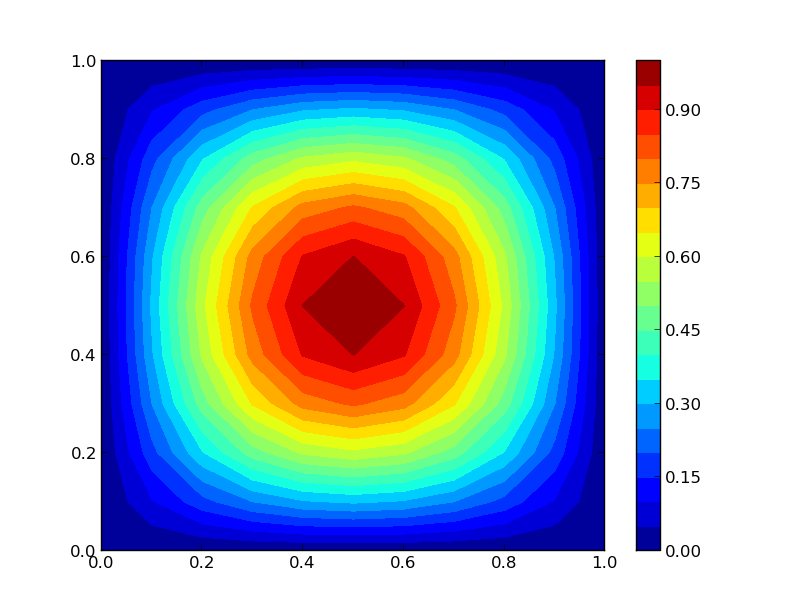
\includegraphics[width=0.7\textwidth]{pix/mesh_example_1}
\end{center}
\end{frame}

\begin{frame}[fragile]
    \frametitle{NumPy}
    \begin{myColorBox}{0.9}{}
\begin{verbatim}
>>> A = np.array( [[1,1], [0,1]] )
>>> B = np.array( [[2,0], [3,4]] )
>>> A*B  # elementwise product
array([[2, 0], 
       [0, 4]])
>>> np.dot(A,B) # matrix product
array([[5, 4],
       [3, 4]])
>>> np.mat(A) * np.mat(B) # matrix product
matrix([[5, 4],
       [3, 4]])
\end{verbatim}
    \end{myColorBox}
There are further functions for array creation, conversions, manipulation, querying, ordering, operations, statistics, basic linear algebra. See NumPy documentation.
\end{frame}

\begin{frame}[fragile]
\frametitle{Numpy}
NumPy subpackages
\begin{itemize}
  \item random: random number generators for various different distributions
  \item linalg: linear algebra tools
  \item fft: discrete Fourier transform
  \item polynomial: efficiently dealing with polynomials
\end{itemize}
\end{frame}

\begin{frame}[fragile]
\frametitle{Numpy}
Example fft:
\begin{myColorBox}{0.9}{}
\begin{verbatim}
>>> sample_rate = 100.0
>>> nsamples = 400
>>> t = np.arange(nsamples) / sample_rate
>>> s = np.cos(2*np.pi*0.5*t) 
+ 0.2*np.sin(2*np.pi*2.5*t+0.1)
>>> S = np.fft.fft(s)
>>> freqs = np.fft.fftfreq(nsamples, 1/samp_rate)
>>> plt.plot(freqs,abs(S))
>>> plt.xlim(-5,5)
>>> plt.show()
\end{verbatim}
\end{myColorBox}
\pause
\begin{center}
      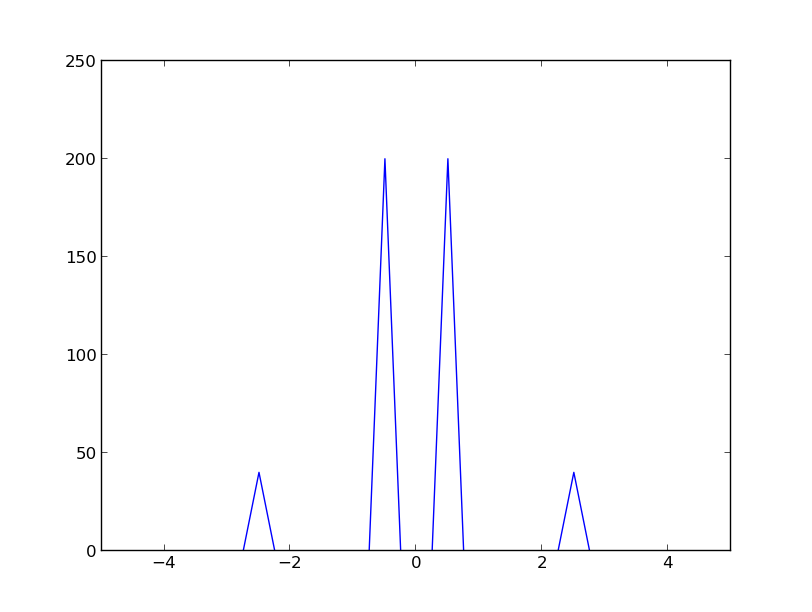
\includegraphics[width=0.5\textwidth]{pix/fft_example_1}
\end{center}
\end{frame}

\begin{frame}
\begin{center}
\Huge{Scipy}
\end{center}
\end{frame}

\begin{frame}
\frametitle{Scipy}
SciPy is a collection of mathematical algorithms and convenience functions built
on the Numpy extension for Python. Scipy subpackages are:
\begin{itemize}
  \item cluster: Clustering algorithms
  \item constants: Physical and mathematical constants
  \item fftpack: Fast Fourier Transform routines
  \item integrate: Integration and ordinary differential equation solvers
  \item interpolate: Interpolation and smoothing splines
  \item io: Input and Output
  \item linalg: Linear algebra
  \item ndimage: N-dimensional image processing
  \item odr: Orthogonal distance regression
  \item optimize: Optimization and root-finding routines
  \item signal: Signal processing
  \item sparse: Sparse matrices and associated routines
  \item spatial: Spatial data structures and algorithms
  \item special: Special functions
  \item stats: Statistical distributions and functions
  \item weave: C/C++ integration               
\end{itemize}
\end{frame}

\begin{frame}[fragile]
\frametitle{Scipy}
Interpolation
\begin{myColorBox}{1.0}{}
\begin{verbatim}
>>> from scipy.interpolate import interp1d
>>> x = np.linspace(0, 10, 10)
>>> y = np.exp(-x/3.0)
>>> f = interp1d(x, y)
>>> f2 = interp1d(x, y, kind='cubic')
>>> xnew = np.linspace(0, 10, 40)
>>> plt.plot(x,y,'o')
>>> plt.plot(xnew,f(xnew),'-',xnew, f2(xnew),'--')
>>> plt.legend(['data', 'linear', 'cubic'], loc='best')
>>> plt.show()
\end{verbatim}
\end{myColorBox}
\pause
\begin{center}
      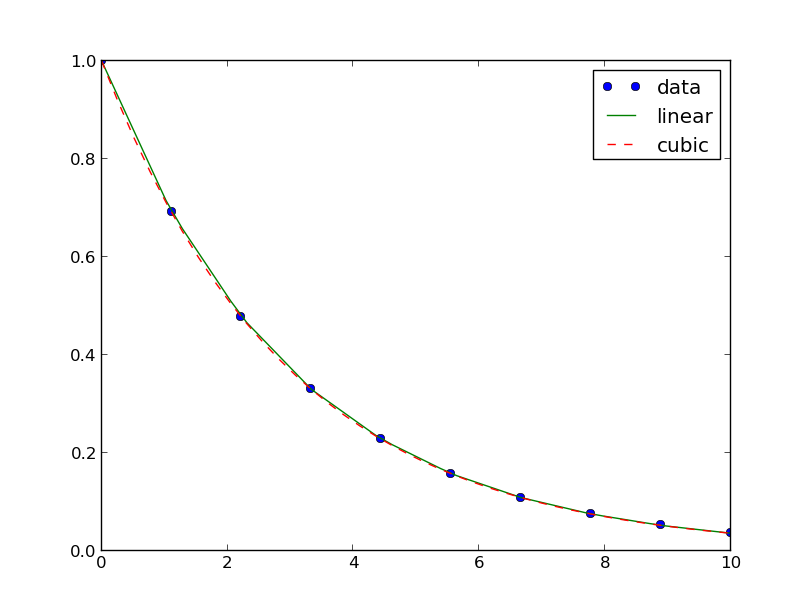
\includegraphics[width=0.5\textwidth]{pix/interpolation_example_1}
\end{center}
\end{frame}

\begin{frame}[fragile]
\frametitle{Scipy}
Least-squares data fitting:
\begin{myColorBox}{1.0}{}
\begin{verbatim}
>>> from scipy import linalg
>>> c1,c2= 5.0,2.0
>>> i = np.arange(1,11)
>>> xi = 0.1*i
>>> yi = c1*np.exp(-xi)+c2*xi
>>> zi = yi + 0.05*np.max(yi)*np.random.randn(len(yi))
# A*c = zi
>>> A = np.array([np.exp(-xi),xi]).T
>>> c,resid,rank,sigma = linalg.lstsq(A,zi)
>>> c
array([ 5.0525305 ,  2.09272423])
>>> resid
0.70716255651624638
\end{verbatim}
\end{myColorBox}
\end{frame}

\begin{frame}[fragile]
\frametitle{Scipy}
\begin{myColorBox}{0.9}{}
\begin{verbatim}
>>> xi2 = np.linspace(0.1,1.0,100)
>>> yi2 = c[0]*np.exp(-xi2) + c[1]*xi2
>>> plt.plot(xi,zi,'x',xi2,yi2)
>>> plt.show()\end{verbatim}
\end{myColorBox}
\pause
\begin{center}
      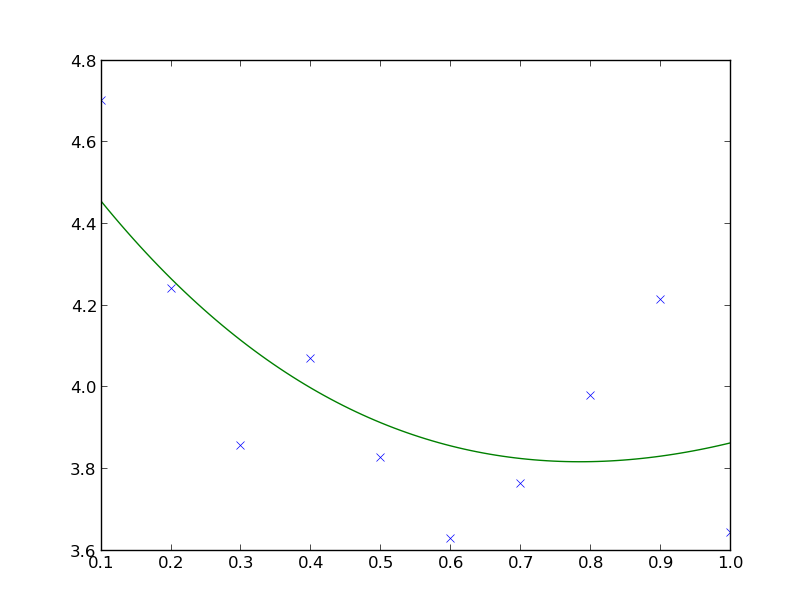
\includegraphics[width=0.5\textwidth]{pix/least_squares_example_1}
\end{center}
\end{frame}

\begin{frame}[fragile]
\frametitle{Scipy}
Loading *.mat files generated by Matlab:
\begin{myColorBox}{1.0}{}
\begin{verbatim}
>> %Matlab
>> mat1 = [1 2 3; 4 5 6; 7 8 9];
>> arr1 = [10 11 12];
>> save test_io.mat mat1 arr1;
\end{verbatim}
\end{myColorBox}
\pause
\begin{myColorBox}{1.0}{}
\begin{verbatim}
>>> from scipy.io import loadmat
>>> a = loadmat('test_io.mat')
>>> a.keys()
['mat1', '__version__', '__header__', 'arr1', ...]
>>>a['mat1']
array([[1, 2, 3],
       [4, 5, 6],
       [7, 8, 9]], dtype=uint8)
>>> a['arr1']
>>> array([[10, 11, 12]], dtype=uint8)
>>> a = loadmat('test_io.mat',squeeze_me=True)
>>> a['arr1']
array([10, 11, 12], dtype=uint8)
\end{verbatim}
\end{myColorBox}
\end{frame}

\begin{frame}[fragile]
\frametitle{Scipy}
\ldots do the reverse:
\begin{myColorBox}{1.0}{}
\begin{verbatim}
>>> from scipy.io import savemat
>>> arr2 = a['arr1']
>>> arr2[0] = 20
>>> savemat('test_io_2.mat',
{'mat1':a['mat1'], 'arr2':arr2},oned_as='row')
\end{verbatim}
\end{myColorBox}
\pause
\begin{myColorBox}{1.0}{}
\begin{verbatim}
>> load test_io_2.mat
>> mat1
mat1 =
    1    2    3
    4    5    6
    7    8    9
>> arr2
arr2 =
   20   11   12
\end{verbatim}
\end{myColorBox}
\end{frame}

\begin{frame}[fragile]
\frametitle{Scipy}
Reading NetCDF files:
\begin{myColorBox}{1.0}{}
\begin{verbatim}
>>> # Reading a GMT grid file
>>> from scipy.io import netcdf
>>> nc = netcdf.netcdf_file('ww3.07121615_GLOBAL05.grd')
>>> nc.variables.keys()
>>> ['y', 'x', 'z']
>>> nc.variables['y'].data
>>> array([-58.5, -58. , -57.5, ..., -31. , -30.5, -30. ])
>>> nc.history
>>> '/usr/local/GMT4.5.7/bin/surface 
-R146.250000/190.000000/-58.500000/-30.000000 
-I0.5 -Gww3.07121615_GLOBAL05.grd 
ww3.07121615_GLOBAL05.xyz'
\end{verbatim}
\end{myColorBox}
\end{frame}

\begin{frame}[fragile]
\frametitle{Documentation}
\begin{itemize}
  \item http://docs.scipy.org/doc/
  \item http://www.scipy.org/Cookbook
  \item http://scipy-central.org/ (code repository)   
\end{itemize}
\end{frame}

\begin{frame}
\begin{center}
\Huge{Exercises}
\end{center}
\end{frame}

\begin{frame}
\begin{center}
\Huge{Basemap and pyproj}
\end{center}
\end{frame}

\begin{frame}
\begin{center}
\Huge{Basemap}
\end{center}
\end{frame}

\begin{frame}
\frametitle{Basemap}
\begin{itemize}
  \item Matplotlib toolkit to plot maps
  \item Does provide facilities to convert coordinates to one of 25 map
  projections (using the PROJ library)
  \item Plotting is done by matplotlib
  \item Inbuild support for shapefiles
\end{itemize}
\end{frame}

\begin{frame}[fragile]
\frametitle{Basemap}
A very simple map:
\begin{myColorBox}{0.9}{}
\begin{verbatim}
>>> from mpl_toolkits.basemap import Basemap
>>> m = Basemap(projection='merc', llcrnrlat= 45.5, 
urcrnrlat=48, llcrnrlon=5, urcrnrlon=12, lat_ts= 47, 
resolution='i')
>>> m.drawcountries()
>>> plt.show()
\end{verbatim}
\end{myColorBox}
\pause
\begin{center}
      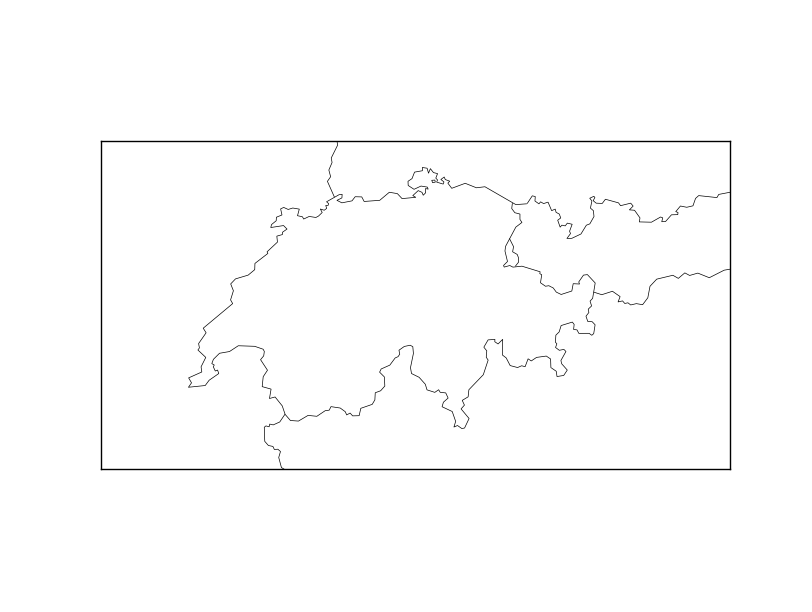
\includegraphics[width=0.8\textwidth]{pix/basemap_example_1}
\end{center}
\end{frame}

\begin{frame}[fragile]
\frametitle{Basemap}
\ldots adding a few details:
\begin{myColorBox}{1.0}{}
\begin{verbatim}
 >>> m.drawcoastlines()
 >>> m.drawcountries(linewidth=1.0)
 >>> m.drawmeridians([6,7,8,9,10,11],labels=[0,0,0,1])
 >>> m.drawparallels([46,46.5,47,47.5],labels=[1,0,0,0])
 >>> m.drawrivers(color='b')
 >>> plt.show()
\end{verbatim}
\end{myColorBox}
\pause
\begin{center}
      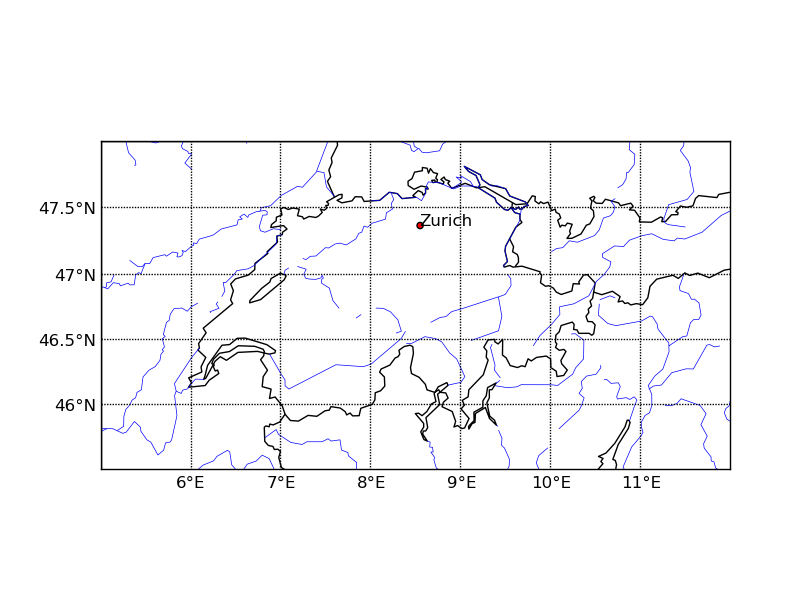
\includegraphics[width=0.8\textwidth]{pix/basemap_example_2}
\end{center}
\end{frame}



\begin{frame}[fragile]
\frametitle {Credits}
    \begin{itemize}
    \item The Python Tutorial (http://docs.python.org/tutorial/)
    \item Sebastian Heimann - The Informal Python Boot Camp (http://emolch.org/pythonbootcamp.html)
    \item Software Carpentry (http://software-carpentry.org/4\_0/python/)
    \item Python Scripting for Computational Science, Hans Petter Langtangen
    \item Matplotlib for Python Developers, Sandro Tosi
    \end{itemize}
\end{frame}

\end{document}
